
\begin{question}
Let's continue conducting a Box-Jenkins procedure for log(gas) time series.

You can load the gas dataset in R by importing forecast library or if you use other programming languages you can download it \href{https://github.com/vincentarelbundock/Rdatasets/blob/master/csv/forecast/gas.csv}{here}.

\begin{figure}[H]
\centering
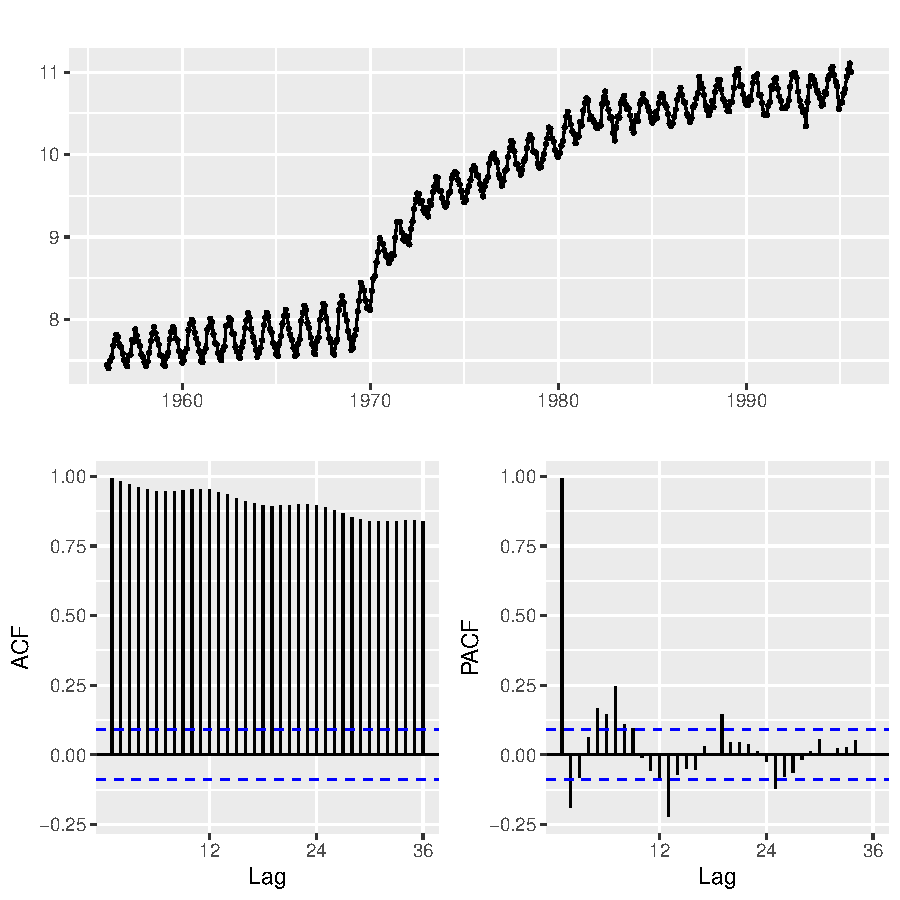
\includegraphics{unnamed-chunk-1-1.pdf}
\caption{plot of chunk unnamed-chunk-1}
\end{figure}

Is the process stationary?
\begin{answerlist}
  \item Yes, we can proceed with log(gas) time series
  \item No, seasonal differencing should be applied
  \item No, first differencing should be applied
  \item No, both first and seasonal differencing should be applied
\end{answerlist}
\end{question}

\begin{solution}
Only if we apply both first and seasonal differences the mean will be stable over time. From analysing the ACF plot it is clear that there is a unit root and a seasonal unit root, but you can also check this using unit root tests.
\end{solution}

